\documentclass[10pt]{article}

\usepackage{spheric}
%%%TITLE
\title{Numerical Simulation of Rayleigh-Taylor Instability by MPS Multiphase Method}
\date{}

%%AFFILIATIONS

\author[$\relax$]{Xiao Wen}
\author[$\relax$]{Decheng Wan$^\dagger$}

\affil[$\relax$]{State Key Laboratory of Ocean Engineering, School of Naval Architecture, Ocean and Civil Engineering, Shanghai Jiao Tong University, Collaborative Innovation Center for Advanced Ship and Deep-Sea Exploration, Shanghai 200240, China}

\affil[$\relax$]{\email{\dagger}{dcwan@sjtu.edu.cn}}


%%DOCUMENT
\begin{document}

\maketitle

%\SelectedTopics{}

%%PLEASE PUT YOUR ABSTRACT HERE
\begin{abstract}
Compared with grid-based methods, the particle method is advantageous for solving multiphase problems with large deformation of the interface between different phases. However, stable multiphase simulations is difficult to be obtained due to the discontinuity of pressure gradient field in the interface and the phenomenon of pressure fluctuation commonly existing in particle method. Therefore, an accurate and stable multiphase model is necessary to be studied.

The paper proposed a multiphase model based on the moving particle semi-implicit method (MPS) for multiphase flows. In this model, the multi-fluids system is treated by a single set of equation and the conservation of volume of both fluids is implicitly satisfied by solving a Poisson pressure equation. A transition region with application of density smoothing technique is introduced to deal with the mathematical discontinuity of density and viscosity in the interface, and the discontinuity of pressure gradient field, which is the main cause of instability in multiphase flows, can be avoided.

To validate this model, one of the classic hydrodynamic instability cases in many natural scenarios and industrial applications, Rayleigh-Taylor instability, is numerical simulated in this paper. At first, different smoothing scheme is adapted in numerical simulation, to test their effects on numerical instability and interface keeping. Then the results are compared with analytical solutions and other numerical methods, proving the stability of this model and the ability of MPS Multiphase method to capture the evolution of the interface between different phases.

\begin{figure}[!htb]
\centering
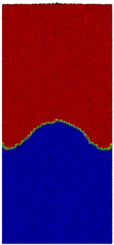
\includegraphics[width=0.275\textwidth]{18-11.png}~~
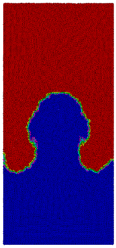
\includegraphics[width=0.275\textwidth]{18-12.png}~~
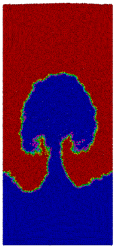
\includegraphics[width=0.275\textwidth]{18-13.png}~~
\caption{The evolution of interface in Rayleigh-Taylor instability simulated by MPS multiphase method: earlier stage (left), middle stage (middle), later stage (right).}\label{fig:18}
\end{figure}

\end{abstract}


%%THE END OF ABSTRACT

%\addbib

\end{document}
